\section*{Lab 4 -- Parallel Processing and SIMD Evaluation}
\addcontentsline{toc}{section}{Lab 4 -- Parallel Processing and SIMD Evaluation}


This assignment is related to \textbf{Lab 4 -- Parallel Processing} and focuses on the exploitation of task-level parallelism on the dual-core ARM Cortex-A9 architecture of the Zybo Z7 board.

The main objective of the laboratory activity is to design and evaluate a shared-memory parallel application in a bare-metal environment, where \textbf{Core~0 (Master)} and \textbf{Core~1 (Worker)} cooperate to perform a vector addition operation. Two input vectors $A$ and $B$ are allocated in shared DDR memory, and the resulting vector $C$ is computed according to:
\[
C[i] = A[i] + B[i]
\]

The workload is evenly partitioned between the two processing cores: Core~0 computes the first half of the vector, while Core~1 processes the second half. Coordination between the cores is achieved through a minimal synchronization mechanism based on shared memory flags (\texttt{start}, \texttt{done0}, \texttt{done1}), without relying on any operating system support.

Execution time is measured using the ARM Cortex-A9 Global Timer, allowing a quantitative comparison between serial and parallel implementations. In addition, the lab investigates the impact of data-level parallelism by enabling compiler auto-vectorization through ARM NEON SIMD instructions.

Overall, this laboratory introduces fundamental concepts of low-level multi-core programming, including explicit workload partitioning, shared-memory communication, synchronization, and performance evaluation in a bare-metal embedded system.


\subsection*{System Debugger Configuration}
\addcontentsline{toc}{subsection}{System Debugger Configuration}

A \textit{System Debugger} run configuration was created in the Xilinx SDK environment.
Before launching the application, the following operations were explicitly enabled in the
\textbf{Target Setup} tab, as required:

\begin{enumerate}
    \item Reset entire system, clearing the FPGA fabric (PL).
    \item Program the FPGA fabric (PL).
    \item Run \texttt{ps7\_init} to initialize the Processing System (PS).
    \item Run \texttt{ps7\_post\_config} to enable level shifters from PL to PS.
\end{enumerate}

In the \textbf{Application} tab:
\begin{itemize}
    \item The \texttt{master.elf} executable was assigned to Processor 0.
    \item The \texttt{worker.elf} executable was assigned to Processor 1.
    \item The options \textit{reset processor} and \textit{stop at program entry} were disabled.
\end{itemize}

This configuration ensures a clean and deterministic execution environment for timing measurements.



\subsection*{Linker Script Modification}

In accordance with the laboratory instructions, the linker script
(\texttt{lscript.ld}) was explicitly modified to ensure correct memory
mapping for the dual-core shared-memory application.

In particular, the DDR memory regions were configured as required so that:
\begin{itemize}
    \item executable code,
    \item global and static data,
    \item stack and heap,
    \item and the shared data structures
\end{itemize}
are all placed in the DDR address space accessible by both processors.

This modification is essential to guarantee correct data sharing between
Core~0 and Core~1 and to avoid memory overlap with private sections
managed by the linker.

Figure~\ref{fig:lab4_lscript} shows the modified linker script used for this laboratory,
which follows the structure and memory layout provided in the lab instructions.

\begin{figure}[h]
    \centering
    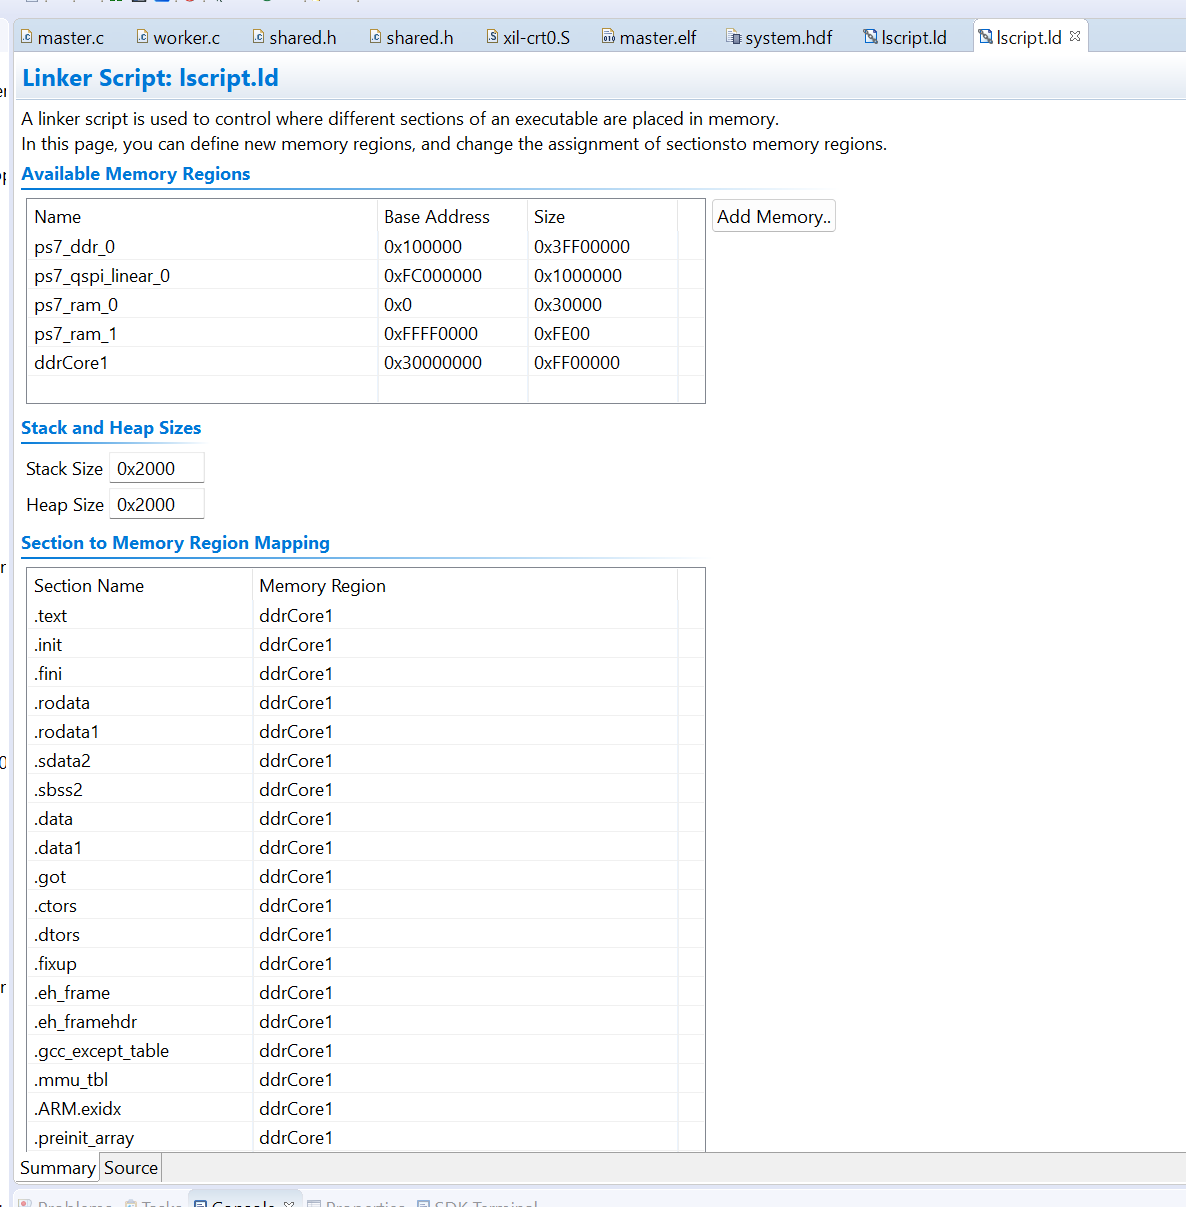
\includegraphics[width=0.95\linewidth]{images/worker_lscript}
    \caption{Modified linker script (\texttt{lscript.ld}) used in Lab~4.}
    \label{fig:lab4_lscript}
\end{figure}

Figure~\ref{fig:lab4_lscript} shows the modified linker script used for this laboratory,
which follows the structure and memory layout provided in the lab instructions.

\begin{figure}[h]
    \centering
    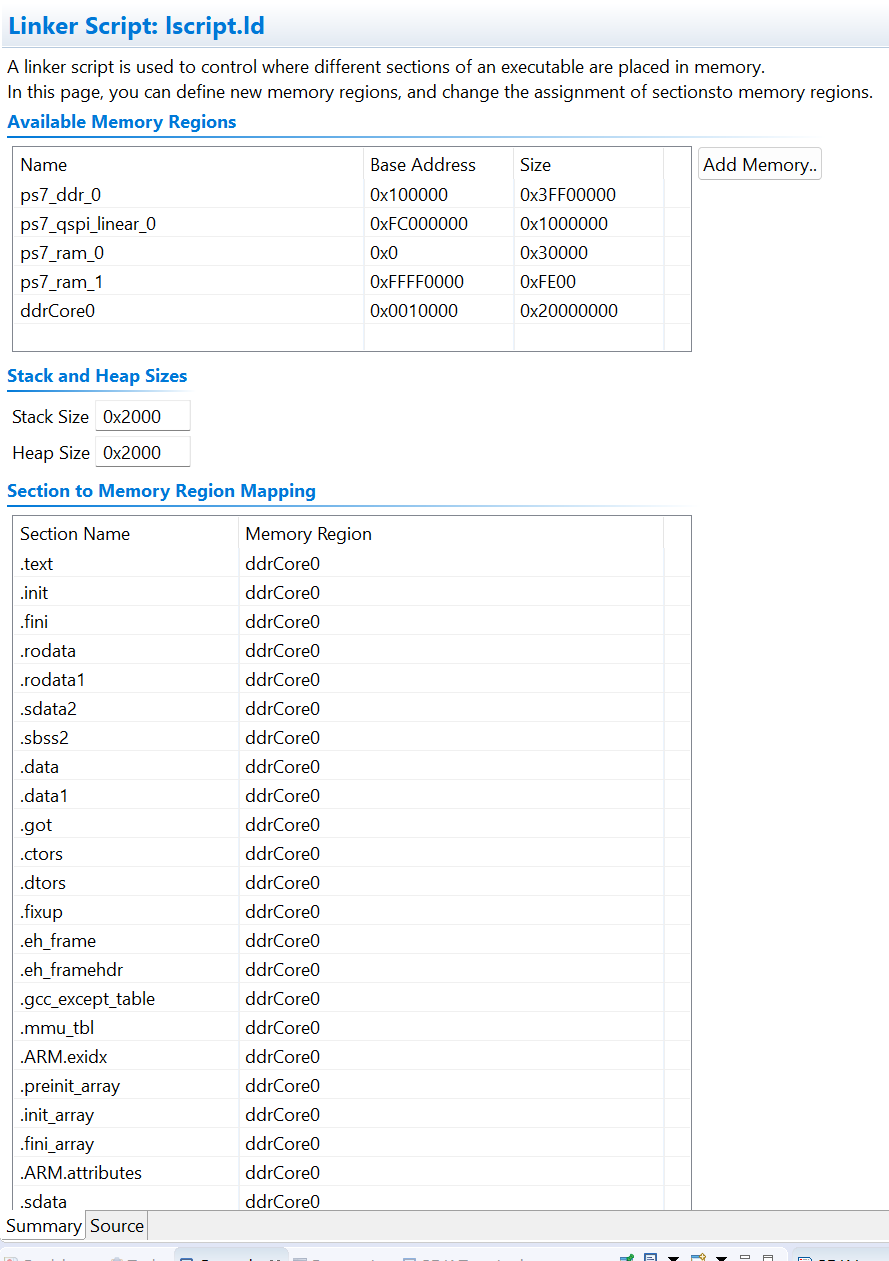
\includegraphics[width=0.95\linewidth]{images/master_lscript}
    \caption{Modified linker script (\texttt{lscript.ld}) used in Lab~4.}
    \label{fig:lab4_lscript}
\end{figure}


\subsection*{Serial Baseline Integration}
\addcontentsline{toc}{subsection}{Serial Baseline Integration}

To evaluate the impact of SIMD optimizations, the following serial reference implementation
was integrated into the master application:

\begin{verbatim}
void vec_add_serial(u32 * restrict c,
                    const u32 * restrict a,
                    const u32 * restrict b,
                    int n)
{
    for (int i = 0; i < n; ++i) {
        c[i] = a[i] + b[i];
    }
}
\end{verbatim}

This function is executed entirely on Processor 0 and is used as a baseline for comparison
with the parallel implementation.

\subsection*{Compilation Settings}
\addcontentsline{toc}{subsection}{Compilation Settings}

Both the \texttt{master} and \texttt{worker} projects were compiled using aggressive optimization
and auto-vectorization flags.

\paragraph{Compiler flags}
\begin{verbatim}
-c -fmessage-length=0 -mcpu=cortex-a9 -mfpu=neon -mfloat-abi=hard
-std=c99 -mvectorize-with-neon-quad -ftree-vectorize
-fopt-info-vec-optimized -fopt-info-vec-missed -ffast-math
\end{verbatim}

\paragraph{Linker flags}
\begin{verbatim}
-mcpu=cortex-a9 -mfpu=neon -mfloat-abi=hard -std=c99
-mvectorize-with-neon-quad -ftree-vectorize
-Wl,-build-id=none -specs=Xilinx.spec
\end{verbatim}

Figures~\ref{fig:master_compiler}--\ref{fig:worker_linker} show the configuration of the
compiler and linker options for both projects.

\begin{figure}[h]
    \centering
    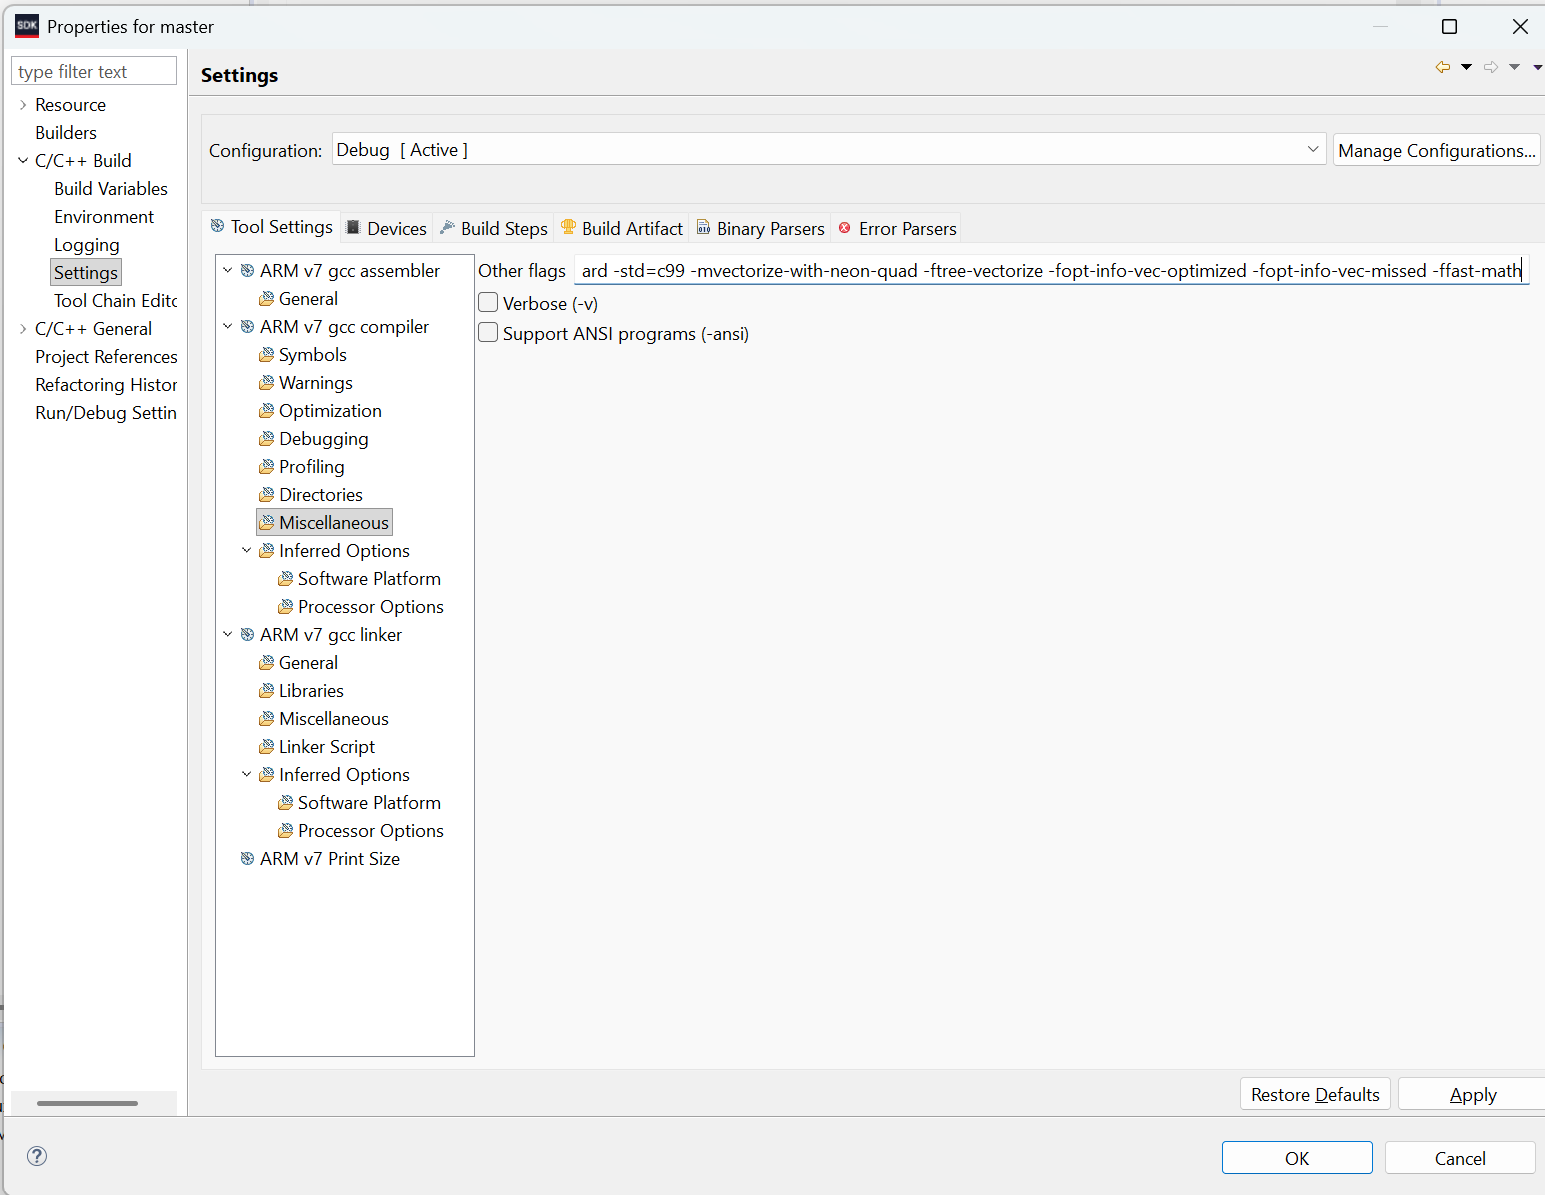
\includegraphics[width=0.9\linewidth]{images/master_compiler.png}
    \caption{Compiler options for the master application.}
    \label{fig:master_compiler}
\end{figure}

\begin{figure}[h]
    \centering
    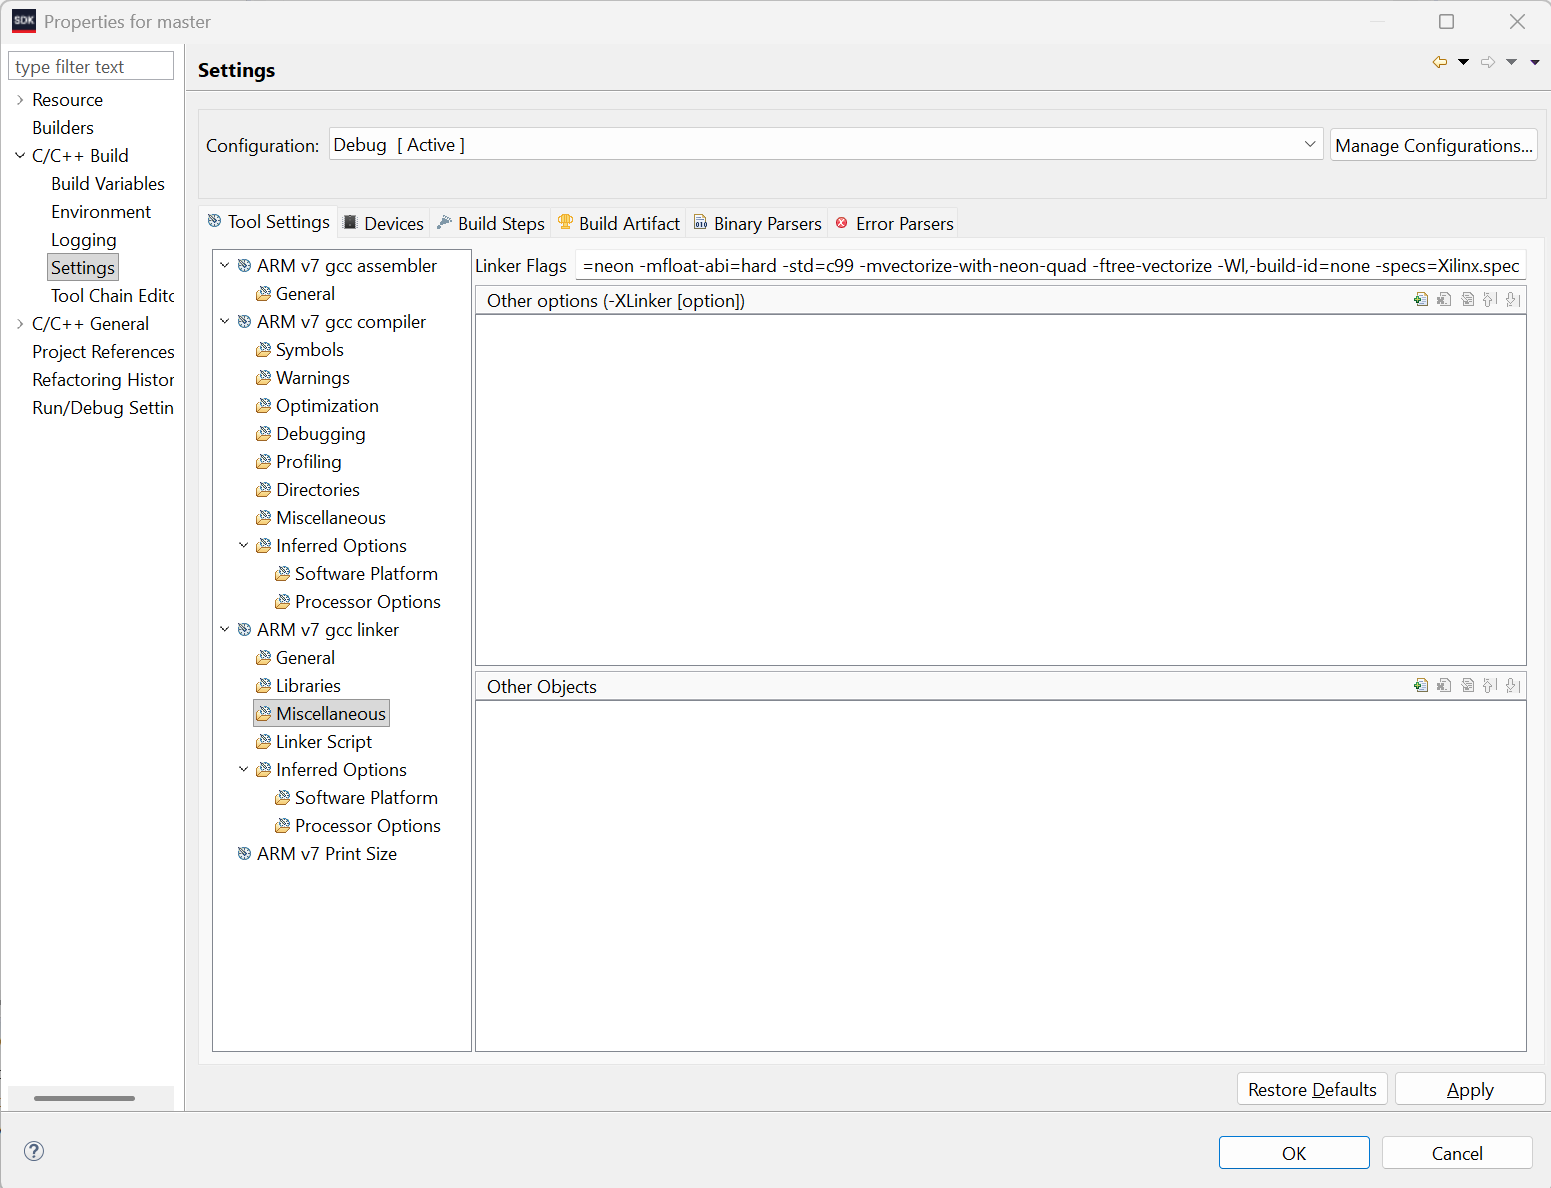
\includegraphics[width=0.9\linewidth]{images/master_linker.png}
    \caption{Linker options for the master application.}
    \label{fig:master_linker}
\end{figure}

\begin{figure}[h]
    \centering
    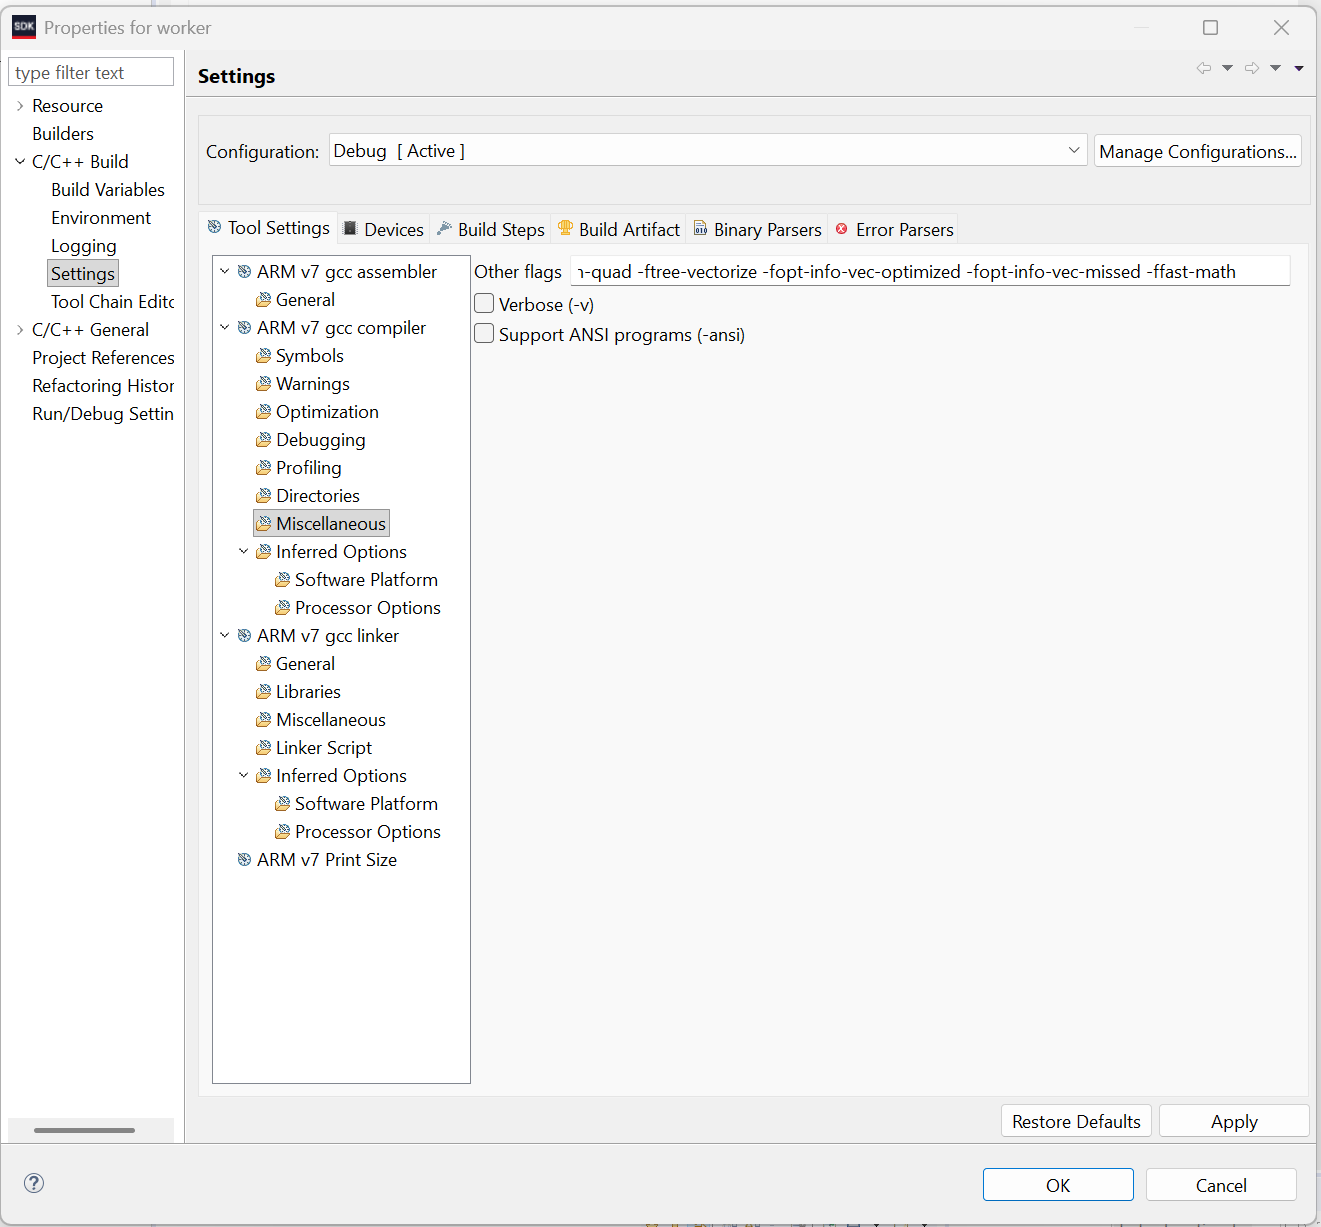
\includegraphics[width=0.9\linewidth]{images/worker_compiler.png}
    \caption{Compiler options for the worker application.}
    \label{fig:worker_compiler}
\end{figure}

\begin{figure}[h]
    \centering
    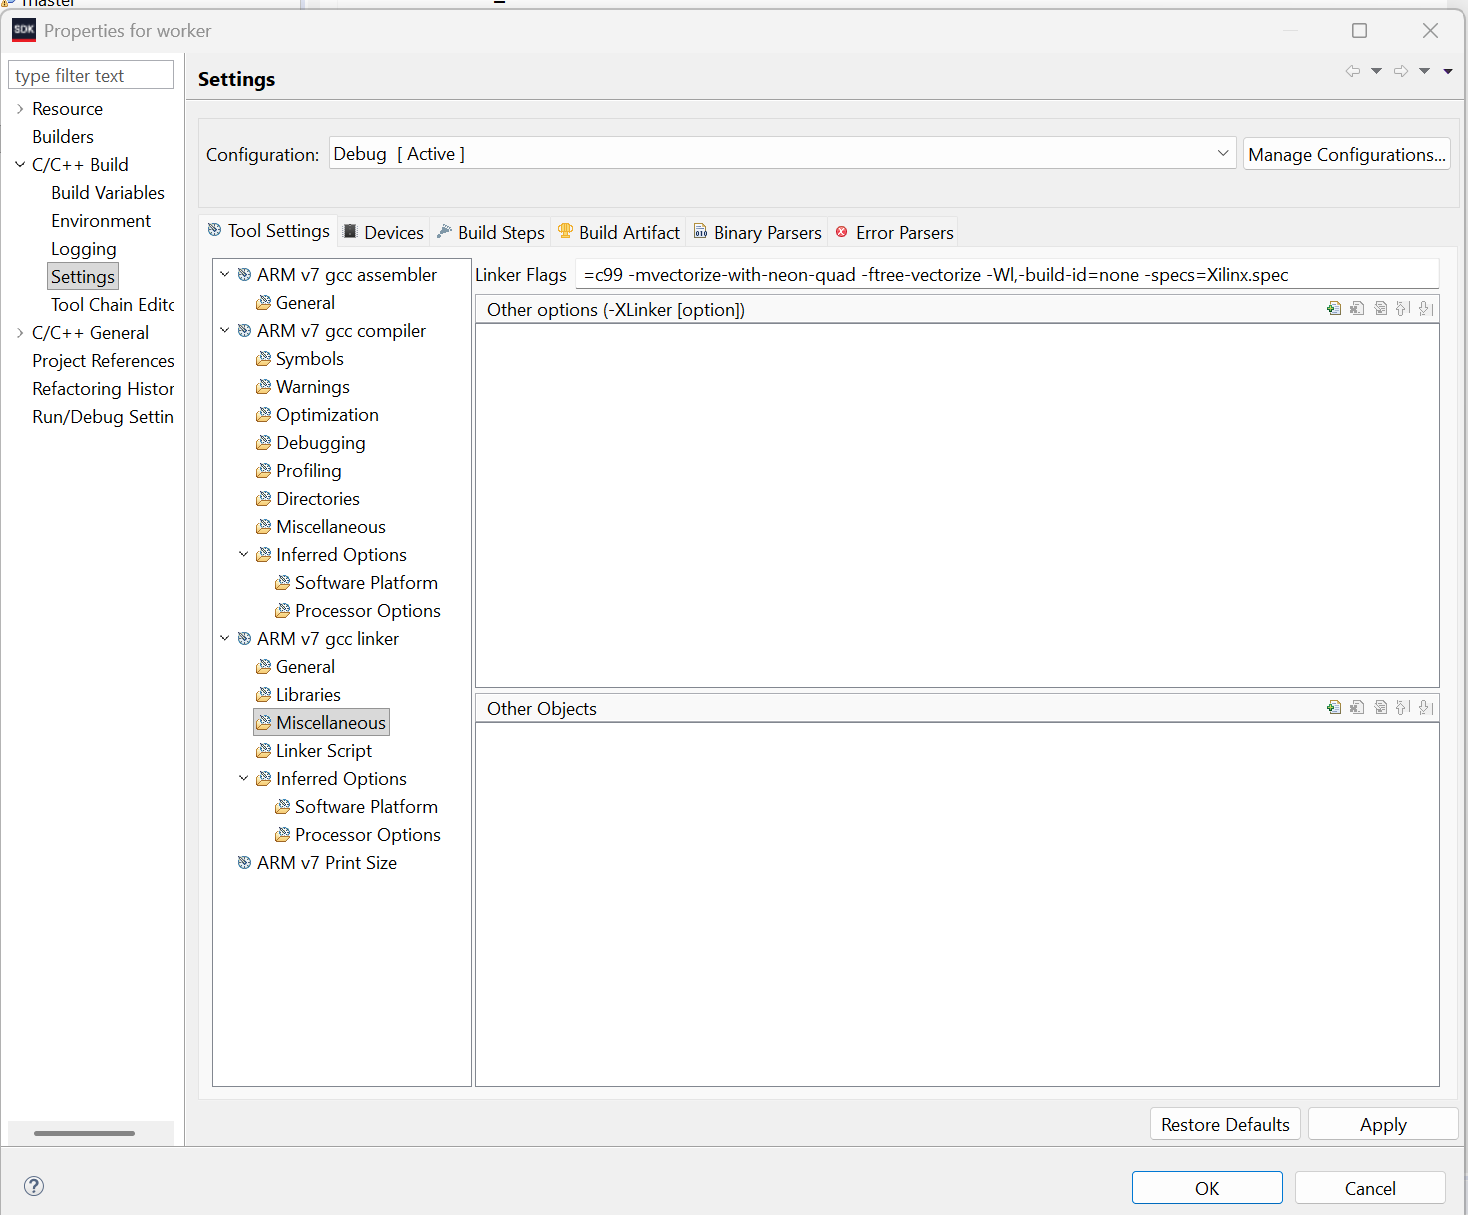
\includegraphics[width=0.9\linewidth]{images/worker_linker.png}
    \caption{Linker options for the worker application.}
    \label{fig:worker_linker}
\end{figure}

\subsection*{Execution Time Measurements}
\addcontentsline{toc}{subsection}{Execution Time Measurements}

Execution time was measured in CPU cycles using the ARM \textit{Global Timer}.
Measurements were performed for different array sizes to study scalability effects.

Figures~\ref{fig:lab4_100}--\ref{fig:lab4_10000} show the UART output for
array sizes of 100, 1000, and 10000 elements, respectively.

\begin{figure}[h]
    \centering
    
\includegraphics[width=0.9\linewidth]{images/lab4_100.png}
    \caption{Execution results for ARRAY\_SIZE = 100.}
    \label{fig:lab4_100}
\end{figure}

\begin{figure}[h]
    \centering
    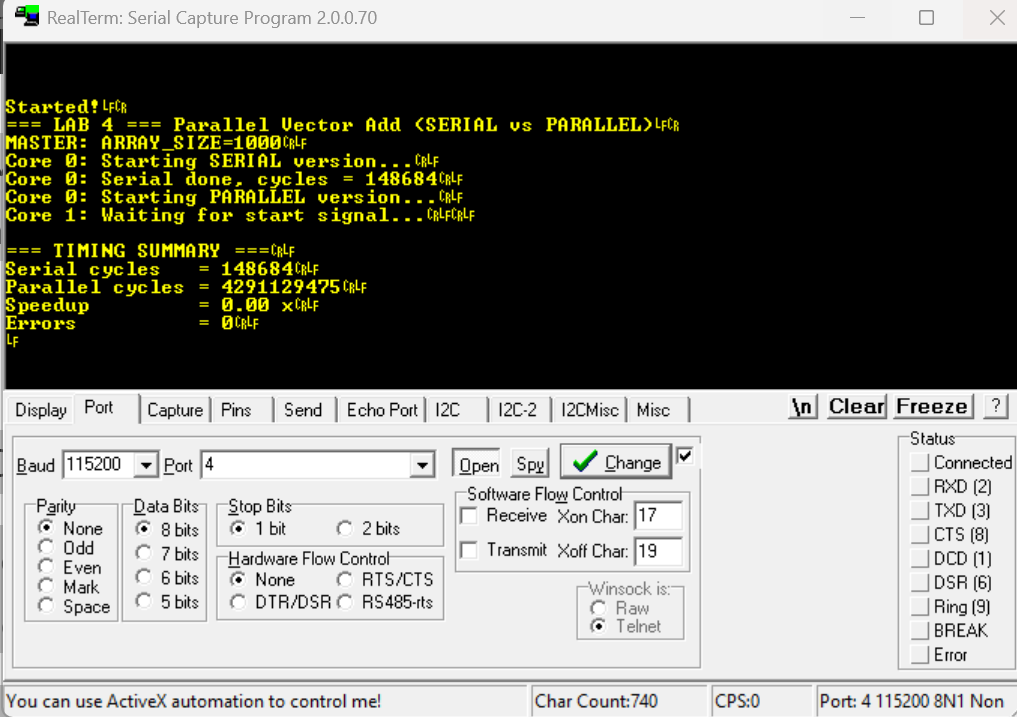
\includegraphics[width=0.9\linewidth]{images/lab4_1000.png}
    \caption{Execution results for ARRAY\_SIZE = 1000.}
    \label{fig:lab4_1000}
\end{figure}

\begin{figure}[h]
    \centering
    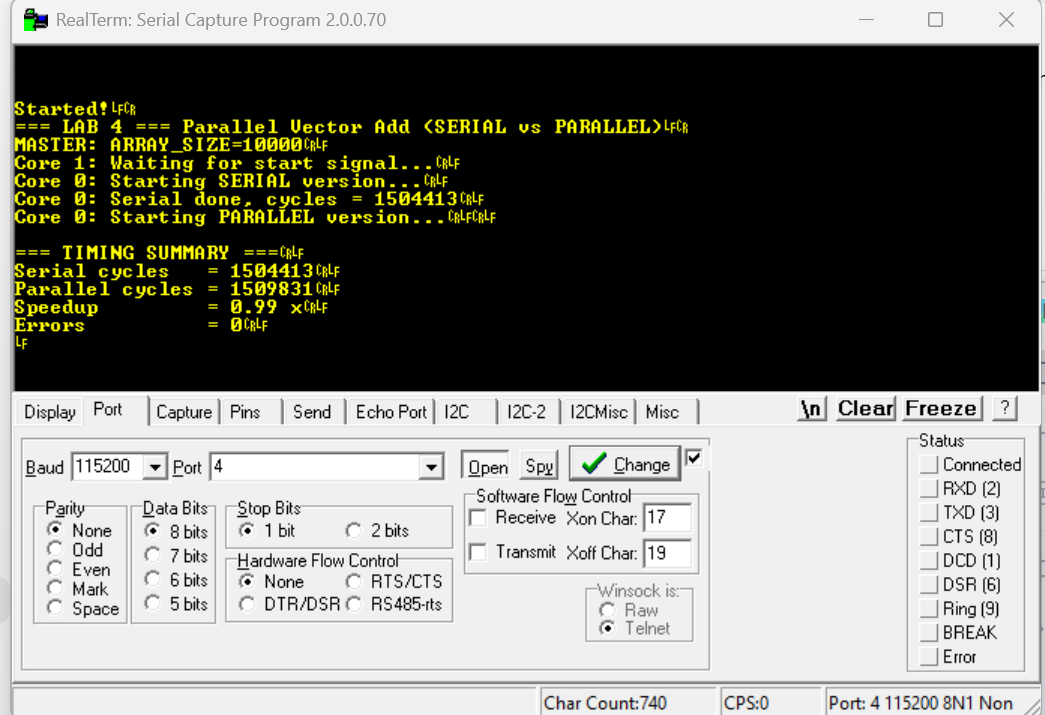
\includegraphics[width=0.9\linewidth]{images/lab4_10000.png}
    \caption{Execution results for ARRAY\_SIZE = 10000.}
    \label{fig:lab4_10000}
\end{figure}

The results show that parallel execution does not provide a significant speedup.
This behavior is expected, as the workload is memory-bound and both processors
contend for the same DDR memory bandwidth.

\subsection*{Assembly Inspection and SIMD Verification}
\addcontentsline{toc}{subsection}{Assembly Inspection and SIMD Verification}

The compiled \texttt{master.elf} file was inspected using the SDK disassembly view.
The analysis confirms that the serial baseline function was successfully
auto-vectorized by the compiler.

In particular, the following NEON instructions are observed:
\begin{itemize}
    \item \texttt{vld1.32} for vector loads,
    \item \texttt{vadd.i32} for vector addition,
    \item \texttt{vst1.32} for vector stores.
\end{itemize}

Figure~\ref{fig:check_neon} highlights the NEON instructions in the disassembled code.

\begin{figure}[h]
    \centering
    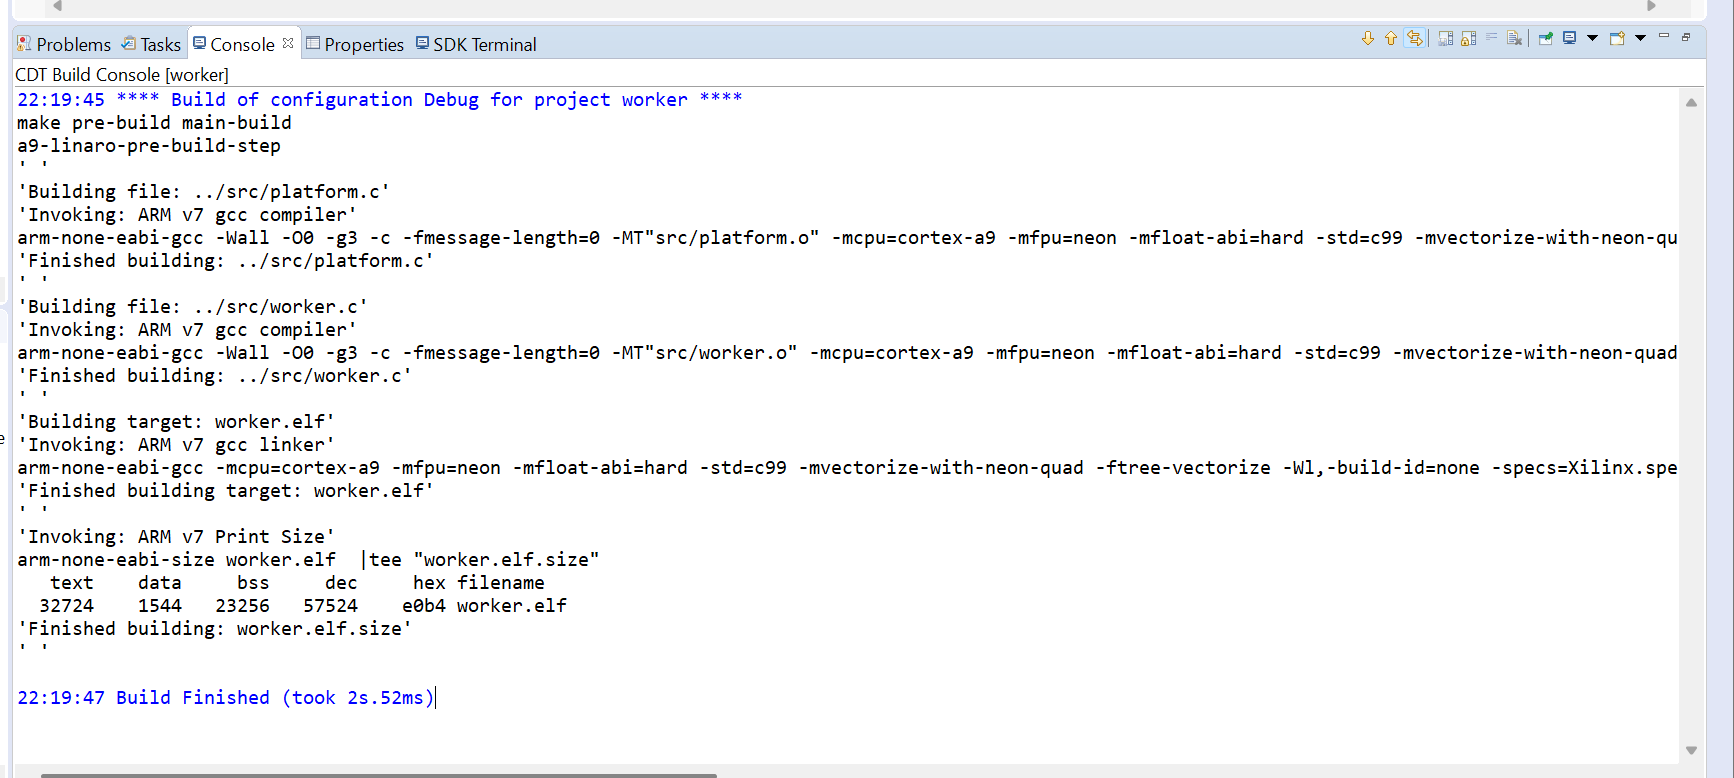
\includegraphics[width=0.95\linewidth]{images/check_neon.png}
    \caption{Disassembly showing NEON vector instructions in the serial implementation.}
    \label{fig:check_neon}
\end{figure}


\subsection*{Conclusions}
\addcontentsline{toc}{subsection}{Conclusions}

This lab demonstrates that:
\begin{itemize}
    \item Parallel execution on multiple cores does not necessarily lead to performance gains
          for memory-bound workloads.
    \item SIMD auto-vectorization using NEON is successfully applied by the compiler and provides
          instruction-level parallelism.
    \item Memory bandwidth and synchronization overhead are the dominant limiting factors in this experiment.
\end{itemize}
